\documentclass{beamer} 
\usetheme{default} 
\usecolortheme{albatross}
\setbeamercovered{transparent}
%\useoutertheme{umbcfootline}  


\usepackage[spanish]{babel}
%\usepackage[latin1]{inputenc}
\usepackage[utf8x]{inputenc}
\usepackage{hyperref}
\usepackage{color}



%\usepackage{multicol}



\title{Entrada y Salida}

\author{Manuel J. Molino Milla \and Luis Molina Garzón}

\date{\today} %

\institute{IES Virgen del Carmen \and Departamento de Informática}




%\beamerdefaultoverlayspecification{<+->}

\begin{document}


\begin{frame}
  \titlepage
\end{frame}

\begin{frame}
    \frametitle{Logo}
\begin{figure}

\includegraphics[scale=1]{imagenes/logo.jpeg} 
\caption{Logo Java}
\end{figure}
\end{frame}

\begin{frame}
  \frametitle{Contenido}
  \tableofcontents[pausesections]
\end{frame}

\section{Clase File}
\begin{frame}
\frametitle{Introducción	}
\begin{description}[<+-|alert@+>]
\item[JDK 1.0] Introduce el paquete \emph{java.io}, I/O basada en stream
\item[JDK 1.4] Introduce el paquete \emph{java.nio}, I/O basada en buffer
\item[JDK 1.5] Introduce I/O de texto formateado con nuevas clases \emph{Scanner}, \emph{Formatter} o \emph{printf}
\item[JDK 1.7] mediante \emph{NIO.2} con I/O no bloqueante.
\end{description}
\pause
\end{frame}


\begin{frame}[fragile]
\frametitle{Class java.io.File (Pre-JDK 7)}
\begin{itemize}[<+->]
\item Representa tanto un fichero como un directorio.
\item Windows usa '\alert{$\backslash$}' como separador de directorio; mientras que  Unix/Mac usan '\alert{/}'
\item Windows usa  '\alert{;}' as como separador de la ruta de archivos, mietras que Unix/Mac usan '\alert{:}'.
\item Windows usa '\alert{$\backslash$r$\backslash$n}' como fin de fichero; mientras que  Unix usa '\alert{$\backslash$n}'  y Mac usa '\alert{$\backslash$r}'.
\item '\alert{C:$\backslash$}' or '\alert{$\backslash$}' es el directorio raíz. Y en Unix/Mac es '\alert{/}'
\item El \emph{path} se puede determinar de forma absoluta \emph{/home/usuario/fichero} o usar \alert{.} o \alert{..} como directorio actual o directorio padre, ejemplo: \emph{./fichero}
\item Constructores:
\end{itemize}
\pause
\begin{footnotesize}
\begin{verbatim}
public File(String pathString)
public File(String parent, String child)
public File(File parent, String child)
// Construyen un File dado el path
  
public File(URI uri)
// Construyen un File con file-URI "file://...."
\end{verbatim}
\end{footnotesize}
\end{frame}



\begin{frame}[fragile]
\frametitle{Ejemplo}
\begin{footnotesize}
\begin{block}{Ejemplos básicos}
\begin{verbatim}
File file = new File("in.txt"); //con ruta relativa
// con ruta abslouta
File file = new File("d:\\myproject\\java\\Hello.java");  
File dir  = new File("c:\\temp");   // Un directorio
\end{verbatim}
\end{block} 
\pause
\begin{block}{Para el caso de una apliación que distribuimos como jar}
\begin{verbatim}
java.net.URL url = this.getClass().getResource("icon.png");
\end{verbatim}
\end{block} 
\end{footnotesize}
\end{frame}


\begin{frame}[fragile]
\frametitle{Verificando propiedades de un archvivo o directorio}
\begin{footnotesize}
\begin{verbatim}
public boolean exists()      // Testea si archvio/directorio existe.
public long length()         // Devuelve la longtud del fichero.
public boolean isDirectory() // Tes directorio.
public boolean isFile()      // Comprueba si es un archivo.
public boolean canRead()     // Comprueba si tiene permiso de lectura.
public boolean canWrite()    // Comprueba si tiene permiso de escritura.
public boolean delete()      // Borra el archivo/directorio.
public void deleteOnExit()   // Borra el archivo/directorio
//cuando el programa finalice..
public boolean renameTo(File dest) // Renombra el archivo.
public boolean mkdir()        // Crea el directorio.
public String[] list()     // Lista el contenido del directorio.
public File[] listFiles()  // Lista el contenido del directorio.
\end{verbatim}
\end{footnotesize}
\end{frame}

\begin{frame}[fragile]
\frametitle{Ejemplo listado recursivo de archivos}
\begin{small}
\begin{verbatim}
import java.io.File;
public class ListDirectoryRecusive {
   public static void main(String[] args) {
      File dir = new File("d:\\myproject\\test");  
      listRecursive(dir);
   }
   
   public static void listRecursive(File dir) {
      if (dir.isDirectory()) {
         File[] items = dir.listFiles();
         for (File item : items) {
            System.out.println(item.getAbsoluteFile());
            if (item.isDirectory()) listRecursive(item);  
         }
      }
   }
}
\end{verbatim}
\end{small}
\end{frame}

\begin{frame}[fragile]
\frametitle{Listado de archivos con filtro}
\begin{verbatim}
public String[] list(FilenameFilter filter)
public File[] listFiles(FilenameFilter filter)
public File[] listFiles(FileFilter filter)
//FileFilter usa el siguiente método:
public boolean accept(File dirName, String fileName)
\end{verbatim}
\end{frame}

\begin{frame}[fragile]
\frametitle{Ejemplo listado recursivo de archivos}
\begin{small}
\begin{verbatim}
// Listar ficheros terminados  ".java"
import java.io.File;
import java.io.FilenameFilter;
public class ListDirectoryWithFilter {
   public static void main(String[] args) {
      File dir = new File(".");   // current working directory
      if (dir.isDirectory()) {
         // List only files that meet the filtering criteria
         //  programmed in accept() method of FilenameFilter.
         String[] files = dir.list(new FilenameFilter() {
            public boolean accept(File dir, String file) {
               return file.endsWith(".java");
            }
         });  // clase interna de FilenameFilter
         for (String file : files) {
            System.out.println(file);
         }
      }
   }
}
\end{verbatim}
\end{small}
\end{frame}

\section{Stream}
\begin{frame}[fragile]
\frametitle{Introducción a los stream}
\begin{itemize}[<+->]
\item Los programas leen datos del teclado, ficheros, de la red, de la memoria, \dots.
\item Luego se envían al monitor, ficheros, a otro programa,\dots.
\item Ej Java la I/O se maneja con \emph{stream}
\item Un \emph{stream} es un flujo secuencial y contiguo de datos.
\item Java recibe los datos mediante un \emph{input stream}
\item Y envía los datos mediante un \emph{ioutput stream}
\item Las operaciones implican tres pasos:
\begin{enumerate}
\item Abrir un input/output stream asociado con un dispositivo físico, construyendo el oportuno stream.
\item Leer desde input stream abierto hasta encontrar el final del stream, o escribir en el output stream abierto (y opcionalmente volcado al buffer -flush-).
\item Cerrar del input/output stream.
\end{enumerate}
\end{itemize}
\end{frame}

\begin{frame}[fragile]
\frametitle{Caracteres stream y byte stream}
Java almacena de forma interna los caracteres usando 16-bit  UCS-2. Pero la fuente de datos puede almacenar usando codificaciones diferentes como US-ASCII, ISO-8859-x, UTF-8, UTF-16, \dots\\
Java necesita diferenciar entre I/O basada en \alert{bytes}: procesamiento I/O raw bytes o binary data y en \alert{caracteres} usando dos bytes.\\
\begin{figure}
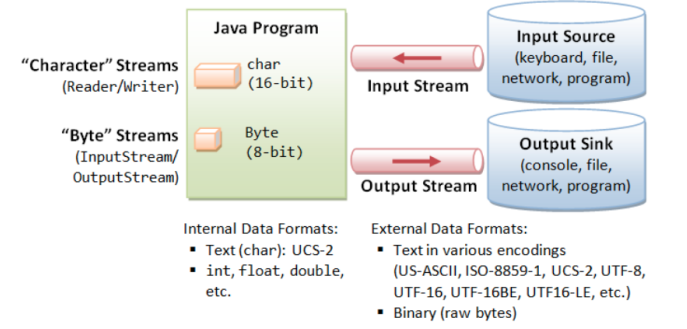
\includegraphics[scale=0.5]{imagenes/stream.png}
\end{figure}
\end{frame}

\subsection{bytes stream}
\begin{frame}
\frametitle{InputStream y OutputStream}
\begin{figure}
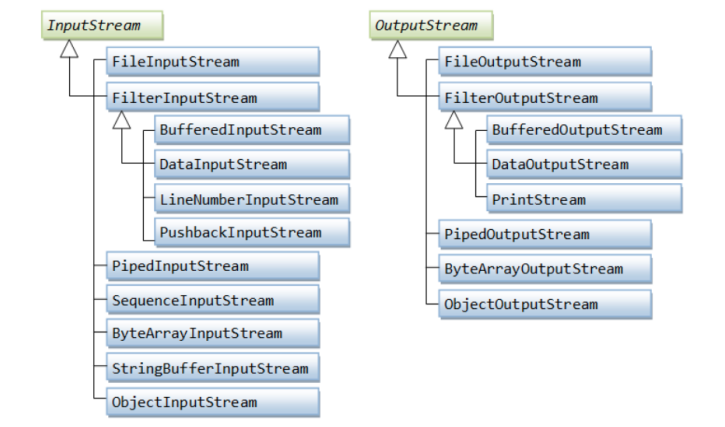
\includegraphics[scale=0.6]{imagenes/io.png}
\end{figure}
\end{frame}

\begin{frame}[fragile]
\frametitle{Leyendo de un InputStream}
La clase \emph{InputStream} es \emph{abstracta} y declara un método \emph{read}:
\begin{quote}
public abstract int read() throws IOException
\end{quote}
\pause
-Devuelve: 
\begin{itemize}[<+->]
\item Los bytes leidos en un rango de 0 a 255.
\item \alert{-1} si detecta el final del stream
\item IOException si hay un error.
\end{itemize}
\pause
Otras variantes de \emph{read}
\begin{verbatim}
public int read(byte[] bytes, int offset, int length) 
    throws IOException
// Lee "length" numero de bytes, almacena desde 
  //el offset del índice.
public int read(byte[] bytes) throws IOException
// Lo mismo que read(bytes, 0, bytes.length)
\end{verbatim}
\end{frame}


\begin{frame}[fragile]
\frametitle{Escribiendo en un OutputStream}
La clase \emph{OutputStream} es \emph{abstracta} y declara un método \emph{write}:
\begin{quote}
public void abstract void write(int unsignedByte)
 throws IOException
\end{quote}
\pause
Otras variantes de \emph{write}
\begin{verbatim}
public void write(byte[] bytes, int offset, int length)
    throws IOException
// Escribe "length" numero de bytes desde el 
//offset del índice.
public void write(byte[] bytes) throws IOException
// Lo mismo que write(bytes, 0, bytes.length)
\end{verbatim}
\end{frame}

\begin{frame}[fragile]
\frametitle{Apertura y cierre de stream}
\begin{small}
Es buena práctica cerrar el \emph{stream} en una clausula \emph{finally}
\begin{verbatim}
FileInputStream in = null;
......  
try {
   in = new FileInputStream(...);  // Open stream
   ......
   ......
} catch (IOException ex) {
   ex.printStackTrace();
} finally {  // always close the I/O streams
   try {
      if (in != null) in.close();
   } catch (IOException ex) {
      ex.printStackTrace();
   }
}
\end{verbatim}
\pause
JDK 1.7 introduce una nueva sintáxis \emph{try-with-resources}, qué automaticamente cierra todos los recursos:
\begin{verbatim}
try (FileInputStream in = new FileInputStream(...)) {
   ......
   ......
} catch (IOException ex) {
   ex.printStackTrace();
}  // Automatically closes all opened resource in try (...).
\end{verbatim} 
\end{small}
\end{frame}

\begin{frame}[fragile]
\frametitle{Flushing  OutputStream}
\begin{quote}
public void flush() throws IOException 
\end{quote}
Fuerza al OutputStream a escribir los datos al dispositivo.
\end{frame}

\begin{frame}[fragile]
\frametitle{Implementación de InputStream/OutputStream}
\emph{InputStream/OutputStream} es una clase abstracta, no se pueden crear objetos de la misma, en función del tipo de dispositivo usaremos la mas conveniente.\\
Ejemplo, para un archivo usaremos \emph{FileInputStream o FileOutputStream}
\end{frame}

\begin{frame}
\frametitle{Encadenando stream}
\begin{figure}
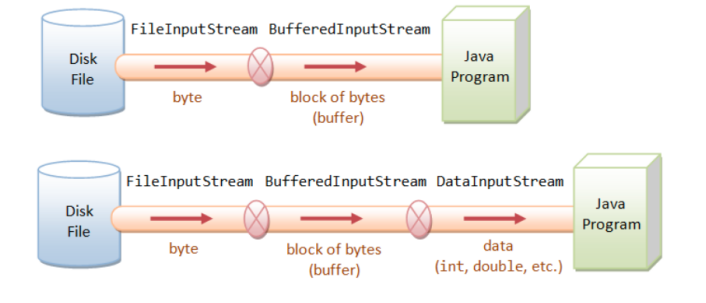
\includegraphics[scale=0.6]{imagenes/encadenado.png}
\end{figure}
\end{frame}

\begin{frame}[fragile]
\frametitle{BufferedInputStream \& BufferedOutputStream}
\begin{itemize}[<+->]
\item Lee byte a byte en cada llamada.
\item El método \emph{read} de InputStream es muy ineficiente.
\item Mejor es usar un bloque de byte en la lectura/escritura.
\item Esto se consigue con un \emph{buffer}
\item Se realiza una operación de I/O desde el dispositivo al buffer de la memoria.
\end{itemize}
\pause
\begin{small}
\begin{verbatim}
FileInputStream fileIn = new FileInputStream("in.dat");
BufferedInputStream bufferIn = new BufferedInputStream(fileIn);
DataInputStream dataIn = new DataInputStream(bufferIn);
// or
DataInputStream in = new DataInputStream(
                      new BufferedInputStream(
                        new FileInputStream("in.dat")));
\end{verbatim}
\end{small}
\end{frame}

\begin{frame}[fragile]
\frametitle{Data-Streams formateados: DataInputStream}
Los usamos cuando estamos leyendos datos primitivos o String.
\pause
\begin{verbatim}
DataInputStream in = new DataInputStream(
                      new BufferedInputStream(
                       new FileInputStream("in.dat")));
\end{verbatim}
\end{frame}

\begin{frame}[fragile]
\frametitle{Métodos de Data-Streams}
\begin{tiny}
\begin{verbatim}
// Para datos primitivos
public final int readInt() throws IOExcpetion;       // Lee 4 bytes 
public final double readDouble() throws IOExcpetion;  // Lee 8 bytes 
public final byte readByte() throws IOExcpetion;
public final char readChar() throws IOExcpetion;
public final short readShort() throws IOExcpetion;
public final long readLong() throws IOExcpetion;
public final boolean readBoolean() throws IOExcpetion;  // Lee 1 byte. 
public final float readFloat() throws IOExcpetion; 
public final int readUnsignedByte() throws IOExcpetion;   // Lee 1 byte [0, 255] 
public final int readUnsignedShort() throws IOExcpetion;  // Lee 2 bytes
[0, 65535]
public final void readFully(byte[] b, int off, int len) throws IOException;
public final void readFully(byte[] b) throws IOException;
 
// Strings
public final String readLine() throws IOException;
     // Lee una línea (hasta nueva línea), 
     convierte cada byte a char - no soporta unicode.
public final String readUTF() throws IOException;
    // lee con String UTF-encoded con los primeros bytes indicando la longitud
    en bytes del UTF
 
public final int skipBytes(int n)  // Salta a número de bytes
\end{verbatim}
\end{tiny}
\end{frame}

\begin{frame}[fragile]
\frametitle{Data-Streams formateados: DataOutputStream}
Los usamos cuando estamos escribiendo datos primitivos o String.
\pause
\begin{verbatim}
DataOutputStream out = new DataOutputStream(
                        new BufferedOutputStream(
                         new FileOutputStream("out.dat")));
\end{verbatim}
\end{frame}

\begin{frame}[fragile]
\frametitle{Métodos de Data-Streams}
\begin{tiny}
\begin{verbatim}
public final void writeInt(int i) throws IOExcpetion;   // escribe 4 bytes
public final void writeFloat(float f) throws IOExcpetion;
public final void writeDoube(double d) throws IOExcpetion; // 
public final void writeByte(int b) throws IOExcpetion;     // 
public final void writeShort(int s) throws IOExcpetion;    // 
public final void writeLong(long l) throws IOExcpetion;
public final void writeBoolean(boolean b) throws IOExcpetion;
public final void writeChar(int i) throws IOExcpetion;
 
// String
public final void writeBytes(String str) throws IOExcpetion;  
public final void writeChars(String str) throws IOExcpetion;
     // Escribe String como UCS-2 16-bit char, Big-endian 
public final void writeUTF(String str) throws IOException;   
     // Escribe String como UTF, 2 bytes indican longitud de UTF bytes 

public final void write(byte[] b, int off, int len) throws IOException
public final void write(byte[] b) throws IOException
public final void write(int b) throws IOException 
\end{verbatim}
\end{tiny}
\end{frame}

\begin{frame}[fragile]
\frametitle{Serialización y Object Streams}
\begin{itemize}[<+->]
\item \emph{ObjectInputStream y ObjectOutputStream} nos permite leer y escribir objetos.
\item Esos objetos pueden ser \emph{ArrayList, Date o cualquier objeto que creemos}
\item La \emph{serialización} es el proceso consistente en convertir un objeto en un flujo de bytes (\emph{stream}).
\item La serialización de un objeto es necesaria bien cuando guardamos el estado del objeto en disco o lo enviámos a través de la red.
\item Para que un objeto se pueda serializar debe implementar una de las dos siguientes interfaces: \emph{java.io.Serializable} o \emph{java.io.Externalizable}
\end{itemize}
\pause
\begin{verbatim}
public final Object readObject() throws IOException, 
   ClassNotFoundException;
public final void writeObject(Object obj) 
   throws IOException;
\end{verbatim}
\end{frame}

\begin{frame}[fragile]
\frametitle{Ejemplos de ObjectInputStream \& ObjectOutputStream}
\begin{verbatim}
ObjectOutputStream out =
   new ObjectOutputStream(
      new BufferedOutputStream(
         new FileOutputStream("object.ser")));
out.writeObject("The current Date and Time is "); 
out.writeObject(new Date());                      
out.flush();
out.close();
\end{verbatim}
\pause
\begin{verbatim}
ObjectInputStream in = 
   new ObjectInputStream(
      new BufferedInputStream(
         new FileInputStream("object.ser")));
String str = (String)in.readObject();
Date d = (Date)in.readObject(new Date());  
in.close();
\end{verbatim}
\end{frame}

\begin{frame}[fragile]
\frametitle{Seriealización}
\begin{itemize}[<+->]
\item Los datos primitivos y array, por defecto son serializables.
\item Los campos estáticos no son serializables.
\item Si queremos que ciertos campos no sean serializables usamos el modificador \emph{trasient}
\item A veces aparece el mensaje \emph{Warning Message "The serialization class does not declare a static final serialVersionUID field of type long" (Advanced)}
\item Debido que algunas clases ya implementan la interfaz \emph{Serializable}
\item Para evitar este mensaje podemos hacer:
\begin{enumerate}
\item Ignorar el mensaje.
\item Añadir un id: \emph{private static final long serialVersionUID = 1L;}
\item Usar la notación $@$SuppressWarnings: \emph{@SuppressWarnings(''serial'')
public class MyFrame extends JFrame \{ ...... \}}
\end{enumerate}
\end{itemize}
\end{frame}

\section{Random Access Files}
\begin{frame}[fragile]
\frametitle{Acceso no secuencial de ficheros}
\begin{itemize}[<+->]
\item Los \emph{stream} que hemos visto o son de escritura o de lectura.
\item También existen \emph{stream} de acceso sencuencial.
\item Valen tanto para la lectura como para la escritura.
\item Lo que nos permiten modificar así como insertar nuevos datos.
\item La clase a usar el la clase \emph{RandomAccessFile}
\item \emph{RandomAccessFile} es como un gran array de bytes. Con un puntero localizado en la posición 0 al abrir el \emph{stream}
\item Dicho puntero avanza con la lectura de un número de bytes.
\end{itemize}
\pause
\begin{figure}
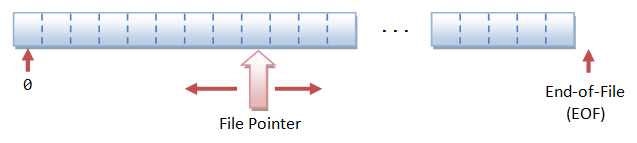
\includegraphics[scale=0.6]{imagenes/random.png}
\end{figure}
\end{frame}

\begin{frame}[fragile]
\frametitle{RandomAccessFile}
\begin{tiny}
\begin{block}{Constructores}
\begin{verbatim}
RandomAccessFile f1 = new RandomAccessFile("filename", "r");
RandomAccessFile f2 = new RandomAccessFile("filename", "rw");
\end{verbatim}
\end{block}
\pause
\begin{block}{Métodos sobre el puntero}
\begin{verbatim}
public void seek(long pos) throws IOException;
// posiciona el puntero en nueva posición.
public int skipBytes(int numBytes) throws IOException;
// Desplaza el puntero una serie de  bytes.
public long getFilePointer() throws IOException;
// Obtiene la posicion del puntero
public long length() throws IOException;
// Devuelve el tamaño del fichero.
\end{verbatim}
\end{block}
\pause
\begin{block}{Métodos de lectura/escritura}
\begin{verbatim}
public int readInt() throws IOException;
public double readDouble() throws IOException;
public void writeInt(int i) throws IOException;
public void writeDouble(double d) throws IOException;
\end{verbatim}
\end{block}
\end{tiny}
\end{frame}

\begin{frame}[fragile]
\frametitle{Ejemplo}
\begin{tiny}
\begin{verbatim}
import java.io.*;
public class TestRandomAccessFile{
  public static void main (String[]args) throws IOException  {
// Create a random-access file
    RandomAccessFile inout = new RandomAccessFile ("inout.dat", "rw");
// Clear the file to destroy the old contents, if any
      inout.setLength (0);
// Write new integers to the file
    for (int i = 0; i < 200; i++)
        inout.writeInt (i);
// Display the current length of the file
      System.out.println ("Current file length is " + inout.length ());
// Retrieve the first number
      inout.seek (0);           // Move the file pointer to the beginning
      System.out.println ("The first number is " + inout.readInt ());
// Retrieve the second number
      inout.seek (1 * 4);       // Move the file pointer to the second number
      System.out.println ("The second number is " + inout.readInt ());
// Retrieve the tenth number
      inout.seek (9 * 4);       // Move the file pointer to the tenth number
      System.out.println ("The tenth number is " + inout.readInt ());
// Modify the eleventh number
      inout.writeInt (555);
// Append a new number
      inout.seek (inout.length ());     // Move the file pointer to the end
      inout.writeInt (999);
// Display the new length
      System.out.println ("The new length is " + inout.length ());
// Retrieve the new eleventh number
      inout.seek (10 * 4);      // Move the file pointer to the next number
      System.out.println ("The eleventh number is " + inout.readInt ());
      inout.close ();
  }
}
\end{verbatim}
\end{tiny}
\end{frame}


\subsection{character stream}
\begin{frame}[fragile]
\frametitle{Character Streams}
\begin{itemize}[<+->]
\item Java usa el conjuto de caracteres 16-bit UCS-2.
\item Pero externamente se pueden guardar con otra codficiación:  US-ASCII, ISO-8859-x, UTF-8, UTF-16, \dots.
\item Independientemente, cuando trabajamos con I/O debemos diferenciar entre procesamiento de \emph{bytes} (raw) o I/O basado en caracteres cuando se procesa texto.
\item Para esto tenemos las clases abstractas \emph{Reader} y \emph{Writer} las cuales implementan los métodos:
\end{itemize}
\pause
\begin{footnotesize}
\begin{verbatim}
public abstract int read() throws IOException
public int read(char[] chars,int offset,int length) throws IOException
public int read(char[] chars) throws IOException
\end{verbatim}
\pause
\begin{verbatim}
public void abstract void write(int aChar) throws IOException
public void write(char[] chars,int offset,int length) throws IOException
public void write(char[] chars) throws IOException
\end{verbatim}
\end{footnotesize}
\end{frame}

\begin{frame}
\frametitle{Reader y Writer}
\begin{figure}
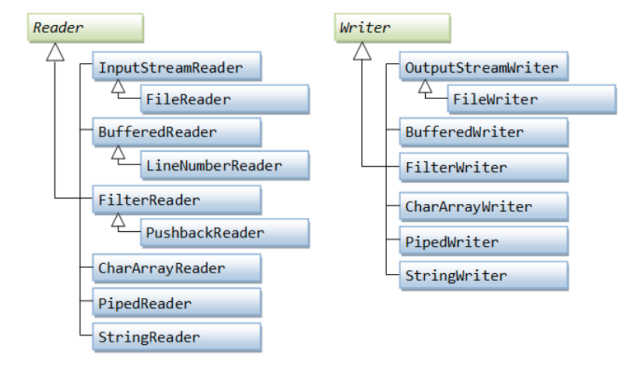
\includegraphics[scale=0.6]{imagenes/rw.png}
\end{figure}
\end{frame}

\begin{frame}[fragile]
\frametitle{FileWriter \& FileReader}
Copiando un fichero de texto:
\begin{footnotesize}
\begin{verbatim}
import java.io.File;
import java.io.FileReader;
import java.io.FileWriter;
import java.io.IOException;

public class Copia {
  public static void main(String[] args)
   throws IOException {
    File inputFile = new File("in.txt");
    File outputFile = new File("out.txt");
    FileReader in = new FileReader(inputFile);
    FileWriter out = new FileWriter(outputFile);
    int c;

    while ((c = in.read()) != -1)
      out.write(c);

    in.close();
    out.close();
  }
}
\end{verbatim}
\end{footnotesize}
\end{frame}

\begin{frame}[fragile]
\frametitle{BufferedReader \& BufferedWriter}
\begin{itemize}[<+->]
\item Se usan para envolver FileWriter y FileReader
\item Mejora el rendimiento de ambos.
\item Pues usamos un buffer de memoria.
\item Además provee un nuevo método \emph{readLine()}
\end{itemize}
\end{frame}

\begin{frame}[fragile]
\frametitle{Ejemplo BufferedReader \& BufferedWriter}
\begin{tiny}
\begin{verbatim}
import java.io.*;
// Write a text message to an output file, then read it back.
// FileReader/FileWriter uses the default charset for file encoding.
public class BufferedFileReaderWriterJDK7 {
   public static void main(String[] args) {
      String strFilename = "out.txt";
      String message = "Hello, world!\nHello, world again!\n";  

      // Print the default charset
      System.out.println(java.nio.charset.Charset.defaultCharset());
 
      try (BufferedWriter out = new BufferedWriter(new FileWriter(strFilename))) {
         out.write(message);
         out.flush();
      } catch (IOException ex) {
         ex.printStackTrace();
      }
 
      try (BufferedReader in = new BufferedReader(new FileReader(strFilename))) {
         String inLine;
         while ((inLine = in.readLine()) != null) {  // exclude newline
            System.out.println(inLine);
         }
      } catch (IOException ex) {
         ex.printStackTrace();
      }
   }
}
\end{verbatim}
\end{tiny}
\end{frame}

\begin{frame}[fragile]
\frametitle{PrintStream \& PrintWriter}
\begin{itemize}[<+->]
\item La clase \emph{PrintStream} y \emph{PrintWriter} se usa para escribir texto formateado bajo \emph{OutputStream}
\item Tenemos métodos como \emph{print}, \emph{printf} o \emph{format}
\end{itemize}
\pause
\begin{small}
\begin{verbatim}
import java.io.*;
public class Print{
        public static void main(String[] arg) throws Exception{
              PrintStream output = new PrintStream(
                 new FileOutputStream(new File("hola.txt")));
              output.println(true);
              output.println((int) 123);
              output.println((float) 123.456);
              output.printf("%.2f %n", 12.3698);
              output.close();
        }
}
\end{verbatim}
\end{small}
\end{frame}

\begin{frame}
\frametitle{PrintStream \& PrintWriter}
\begin{figure}
\includegraphics[scale=0.8]{imagenes/PW.png}
\end{figure}
\end{frame}

\begin{frame}[fragile]
\frametitle{Problemas de codificación}
Lectura de un fichero con codificación iso-8859-1
\begin{verbatim}
try (BufferedReader in = new BufferedReader(
     new InputStreamReader(
         new FileInputStream("prueba2.txt"), "iso-8859-1"));) {
            String linea;
            while ((linea = in.readLine()) != null)
                  System.out.println(linea);
} catch (IOException e) {
         e.printStackTrace();
}
\end{verbatim}
Para una escritura
\begin{verbatim}
BufferedWriter out = new BufferedWriter(
  new OutputStreamWriter(
     new FileOutputStream("prueba3.txt"), "iso-8859-1"))
\end{verbatim}
\end{frame}




\section{I/O Formateado}
\begin{frame}[fragile]
\frametitle{Clase Scanner}
\begin{itemize}[<+->]
\item JDK 1.5 introduce java.util.Scanner.
\item Parsea tokens usando diferentes métodos \emph{nextInt(), nextByte(), nextShort(), nextLong(), nextFloat(), nextDouble(), nextBoolean(), next() for String, y nextLine()}
\item Existen métodos \emph{hasNextXxx()} para chequear la disponibilidad de la entrada.
\end{itemize}
\end{frame}


\begin{frame}[fragile]
\frametitle{Clase Scanner}
\begin{tiny}

\begin{block}{Constructores}
\begin{verbatim}
public Scanner(File source) throws FileNotFoundException
public Scanner(File source, String charsetName) throws FileNotFoundException
// Para System.in
public Scanner(InputStream source)
public Scanner(InputStream source, String charsetName)
// para un String
public Scanner(String source)
\end{verbatim}
\end{block}
\pause
\begin{block}{Ejemplo}
\begin{verbatim}
// Construye un Scanner para parsear un int desde teclado
Scanner in1 = new Scanner(System.in);
int i = in1.nextInt();
 
// Construye un Scanner para parsear los dobles de un fichero
Scanner in2 = new Scanner(new File("in.txt"));   FileNotFoundException
while (in2.hasNextDouble()) {
   double d = in.nextDouble();
}
 
// Construye un Scanner para parsear  string
Scanner in3 = new Scanner("This is the input text String");
while (in3.hasNext()) {
   String s = in.next();
}
\end{verbatim}
\end{block}
\end{tiny}
\end{frame}

\begin{frame}[fragile]
\frametitle{Scanner y el método useDelimiter()}
\begin{itemize}[<+->]
\item \emph{useDelimiter (pattern)}
\item Establece el delimitador para crear \emph{tokens}
\item Ejemplo:
\end{itemize}
\pause
\begin{footnotesize}
\begin{verbatim}
import java.util.Scanner;

public class ScannerTokenizingText {
   public static void main(String[] args) {
      String text = "4231, Java Programming, 1000.00";
      Scanner scanner = new Scanner(text).useDelimiter("\\s*,\\s*");
      int checkNumber = scanner.nextInt();
      String description = scanner.next();
      float amount  = scanner.nextFloat();
      System.out.printf("/***** Tokenizing Text *****/\n\n");
      System.out.printf("String to tokenize: %s\n", text);
      System.out.printf("checkNumber: %d\n", checkNumber);
      System.out.printf("description: %s\n", description);
      System.out.printf("amount: %f", amount);
   }
}
\end{verbatim}
\end{footnotesize}
\end{frame}

\begin{frame}[fragile]
\frametitle{String.format}
\begin{itemize}[<+->]
\item Su compartamiento es similar al de \emph{printf}
\item Se usa un \emph{patrón de formateo}
\item Los parámetros separados por comas.
\item Ejemplos:
\end{itemize}
\pause
\begin{footnotesize}
\begin{verbatim}
int edad = 28;
String nombre = "David";
String patron = "El nombre de la persona es %s y tiene %d años";
String resultado = String.format(patron,nombre,edad);
System.out.print(resultado)  
//El nombre de la persona es David y tiene 28 años
\end{verbatim}
\pause
\begin{verbatim}
int hora = 13;
int minutos = 45;
String nombre = "David";
String patron = "%s ha accedido a las %d:%d h";
String resultado = String.format(patron,nombre,hora,minutos);
System.out.print(resultado);
// David ha accedido a las 13:45 h
\end{verbatim}
\end{footnotesize}
\end{frame}

\section{File I/O in JDK 1.7}
\subsection{Interface java.nio.file.Path}
\begin{frame}[fragile]
\frametitle{Helper class java.nio.file.Paths}
\begin{verbatim}
public static Path get(String first, String... more)
// Este método acepta varios argumentos).
// Los une formanod un objeto Path.
// La locat¡lizació del Path puede o no existir.  
  
public static Path get(URI uri)
// Convierte el URI a un objeto Path.
\end{verbatim}
Ejemplos:
\begin{verbatim}
Path p1 = Paths.get("in.txt");     
Path p2 = Paths.get("c:\\myproejct\\java\\Hello.java");  
Path p3 = Paths.get("/use/local");  
\end{verbatim}
\end{frame}

\begin{frame}[fragile]
\frametitle{Ejemplo}
\begin{tiny}
\begin{verbatim}
import java.nio.file.*;
public class PathInfo {
   public static void main(String[] args) {
      // Windows
      Path path = Paths.get("D:\\myproject\\java\\test\\Hello.java");
      // Unix/Mac
      //Path path = Paths.get("/myproject/java/test/Hello.java");
 
      // Print Path Info
      System.out.println("toString:    " + path.toString());    // D:\myproject\java\test\Hello.java
      System.out.println("getFileName: " + path.getFileName()); // Hello.java
      System.out.println("getParent: " + path.getParent());     // D:\myproject\java\test
      System.out.println("getRoot: " + path.getRoot());         // D:\
 
      // root, level-0, level-1, ...
      int nameCount = path.getNameCount();
      System.out.println("getNameCount: " + nameCount);   // 4
      for (int i = 0; i < nameCount; ++i) {
         System.out.println("getName(" + i + "): " + path.getName(i)); // (0)myproject, (1)java,
      }                                                                // (2) test, (3) Hello.java
      System.out.println("subpath(0,2): " + path.subpath(0,2));  // myproject\java
      System.out.println("subpath(1,4): " + path.subpath(1,4));  // java\test\Hello.java
   }
}
\end{verbatim}
\end{tiny}
\end{frame}

\begin{frame}[fragile]
\frametitle{Helper Class java.nio.file.Files}
\begin{tiny}
\begin{verbatim}
public static long size(Path path)  // Returns the size of the file
 
public static boolean exists(Path path, LinkOption... options)
// Verificas si el Path existse como un file/directory/symlink.
// si devuelve false si el file no existe
// LinkOption especifica como symlink deberían se meneados, 
//   ejmplo: NOFOLLOW_LINKS: no seguir enlaces.
public static boolean notExists(Path path, LinkOption... options)     // ¿Existe?
 
public static boolean isDirectory(Path path, LinkOption... options)   // ¿Directorio?
public static boolean isRegularFile(Path path, LinkOption... options) // ¿Fichero?
public static boolean isSymbolicLink(Path path)                       // ¿Enlace?
 
public static boolean isReadable(Path path)    // ¿permiso lectura?
public static boolean isWritable(Path path)    // ¿permiso escritura?
public static boolean isExecutable(Path path)  // ¿permiso ejecuión?
\end{verbatim}
\end{tiny}
\end{frame}

\begin{frame}[fragile]
\frametitle{Otros métodos}
\begin{verbatim}
public static void delete(Path path) throws IOException
public static boolean deleteIfExists(Path path)
   throws IOException
\end{verbatim}
\pause
\begin{verbatim}
public static Path copy(Path source, Path target, 
   CopyOption... options) throws IOException
public static Path move(Path source, Path target, 
   CopyOption... options) throws IOException
\end{verbatim}
CopyOption: REPLACE\_EXISTING, COPY\_ATTRIBUTES, NOFOLLOW\_LINKS
\pause
\end{frame}

\begin{frame}[fragile]
\frametitle{Otros métodos}
\begin{scriptsize}

\begin{verbatim}
public static byte[] readAllBytes(Path path) throws IOException
// Lee todos los bytes y devuelve byte[]. 
public static Path write(Path path, byte[] bytes,
   OpenOption... options) throws IOException
// Opciones spn: CREATE, TRUNCATE_EXISTING, y WRITE
\end{verbatim}
\pause
\begin{verbatim}
public static List<String> readAllLines(Path path, Charset cs)
    throws IOException
// Lee todas las líneas.
// Terminador de línea puede ser "\n", "\r\n" or "\r".
public static Path write(Path path, Iterable<? extends CharSequence> lines, 
   Charset cs, OpenOption... options) throws IOException
\end{verbatim}

\end{scriptsize}%\pause
\end{frame} 	

\begin{frame}[fragile]
\frametitle{Crear ficheros, directorios o enlaces}
\begin{footnotesize}
\begin{verbatim}
ppublic static Path createFile(Path path, FileAttribute<?>... attrs)
// Crea un nuevo fichero.

public static Path createDirectories(Path dir, FileAttribute<?>
   ... attrs) throws IOException
// Crea un nuevo directorio.

public public static Path createSymbolicLink(Path link, Path target,
   FileAttribute<?>... attrs) throws IOException
// Creates un enlace simbólico
\end{verbatim}
\end{footnotesize}
\end{frame}

\begin{frame}
\frametitle{FIN}
\begin{figure}

\includegraphics[scale=0.35]{imagenes/fing.jpg}
\end{figure}
\end{frame}

\end{document}